\usepackage[english]{babel}
\usepackage{caption}
\captionsetup{labelformat=empty,labelsep=none}
\usepackage{verbatim}
\usepackage{listings}
\usepackage{ulem}
\lstset{language=Perl,basicstyle=\normalsize,tabsize=3,showstringspaces=false}

\title{DBIx::Class Training}
\author{Stefan Hornburg (Racke), Peter Mottram (SysPete)}
\date{Perl Dancer Conference 2015, Vienna, 20th October 2015}

\begin{document}
\maketitle

\input sponsors.tex

\begin{frame}
  \titlepage
\end{frame}

\cleardoublepage

\tableofcontents

\cleardoublepage

\section{Introduction}

\begin{frame}{SQL is ...}
\begin{itemize}
\item SQL is ... boring
\item SQL is ... complex
\item SQL is ... incompatible
\end{itemize}
\end{frame}

\begin{frame}{Complex SQL query}
% add example for complex SQL query
\end{frame}

\begin{frame}{Squeeze OO}
% OO supplied by DBIx::Class
% DBIx::Class + Moo

Object relationship manager (ORM)
SQL => OO
hashref => 

\end{frame}

Just for the fun it, later you will learn how do you
use DBIx::Class to retrieve hash references instead of
objects!

\begin{frame}{DBIx::Class to the rescue!}
% DBIx::Class
\end{frame}

\begin{frame}{Business Logic}
% move business logic into schema
\end{frame}

\subsection{Starting with DBIx::Class}

\begin{frame}{Starting with DBIx::Class}
\begin{itemize}
\item Existing project
\item New project
\end{itemize}
\end{frame}

\subsubsection{Existing Project}

You can use \verb|dbicdump| to create a ``boilerplate'' schema from the
existing database.

\begin{frame}[fragile]{dbicdump}
\begin{lstlisting}
dbicdump -o dump_directory=/home/dance/TravelDance/lib 
         TravelDance::Schema 
         dbi:Pg:dbname=perldance
\end{lstlisting}
\end{frame}

\verb|dbicdump| also provides additional options, e.g.
including \verb|DBIx::Class| components, which we cover
later in the training.

\begin{frame}[fragile]{dbicdump with Components}
\begin{lstlisting}
dbicdump -o dump_directory=/home/dance/TravelDance/lib 
         -o components='["InflateColumn::DateTime"]'
         TravelDance::Schema 
         dbi:Pg:dbname=perldance
\end{lstlisting}
\end{frame}

\subsubsection{Creating database}
Starting a new project involves creating a database, which
isn't as simple as you would think.

MySQL databases should be created with UTF8 encoding and appropriate 
collation for your local, for example:

\begin{frame}[fragile]{Creating MySQL database}
\begin{lstlisting}
    CREATE DATABASE "my_shop_db"
        DEFAULT CHARACTER SET utf8
        DEFAULT COLLATE utf8_general_ci;
\end{lstlisting}
\end{frame}

The following L<Connection attributes|DBIx::Class::Storage::DBI/DBIx::Class specific connection attributes> are recommended as a minimum for MySQL:

\begin{frame}[fragile]{MySQL Connection attributes}
\begin{lstlisting}
    mysql_enable_utf8 => 1,
    on_connect_do     => [
        q|SET SQL_MODE = CONCAT('ANSI,TRADITIONAL,', @@sql_mode)|,
        q|SET SQL_AUTO_IS_NULL = 0|,
    ],
\end{lstlisting}
\end{frame}

NOTE: we no longer recommend the use of 
\verb|on_connect_call =>'set_strict_mode'| since that also forces MySQL's 
\href{https://dev.mysql.com/doc/refman/5.0/en/sql-mode.html#sqlmode\_only\_full\_group\_by}{ONLY\_FULL\_GROUP\_BY} mode which prevents us from using GROUP BY on PK columns which is a great performance boost for PostgreSQL.

=head1 PostgreSQL

PostgreSQL databases should be created with UT8 encoding, for example:

\begin{frame}[fragile]{Creating PostgreSQL database}
\begin{lstlisting}
    createdb -E UTF8 my_shop_db
\end{lstlisting}
\end{frame}

The following L<Connection attributes|DBIx::Class::Storage::DBI/DBIx::Class specific connection attributes> are recommended as a minimum for PostgreSQL:

\begin{frame}[fragile]{PostgreSQL Connection attributes}
\begin{lstlisting}
    pg_enable_utf8 => 1,
    on_connect_do  => 'SET client_min_messages=WARNING;',
\end{lstlisting}
\end{frame}

\section{DBIC Classes}

\begin{frame}{DBIC Classes}
\begin{itemize}
\item Two mandatory types of class
\item One schema class
\begin{itemize}
\item TravelDance::Schema
\end{itemize}
\item One result class for each table
\begin{itemize}
\item TravelDance::Schema::Result::Country
\item TravelDance::Schema::Result::Location
\item TravelDance::Schema::Result::User
\end{itemize}
\end{itemize}
\end{frame}

\subsection{Schema Class}

Here we see the minimal DBIx::Class schema definition:

\begin{frame}[fragile]{Schema Class}
\begin{lstlisting}
package TravelDance::Schema;
use warnings;
use strict;
use base 'DBIx::Class::Schema';

__PACKAGE__->load_components();
1;
\end{lstlisting}
\end{frame}

\verb|load_components| searches \verb|TravelDance::Schema::Result{Set}::*|
for Result and ResultSet classes and loads them into the schema.

\subsection{Result Classes}

\begin{frame}{Result Classes}
\begin{itemize}
\item Need one result class for each table
\item Country => countries
\item Location => locations
\item User => users
\end{itemize}
\end{frame}

\subsubsection{Result Class Definition}
Describes each result class and the database table behind it. 

See \href{https://metacpan.org/pod/DBIx::Class::ResultSource}{DBIx::Class::ResultSource} for more details.

\begin{frame}{Result Class Definition}

\begin{itemize}
\item Table name
\item Columns
\item Primary key
\item Relationships
\end{itemize}
\end{frame}

\subsection{Country Result Class}

\begin{frame}[fragile]{Country / Vanilla DBIx::Class}
\begin{lstlisting}
package TravelDance::Schema::Result::Country;
use base qw/DBIx::Class::Core/;
__PACKAGE__->add_columns(
    country_iso_code => {
        data_type => "char",
        size      => 2,
    },
    name => {
        data_type => "varchar",
        size      => 255,
    },
);
\end{lstlisting}
\end{frame}

\begin{frame}[fragile]{Country / Vanilla DBIx::Class}
\begin{lstlisting}
__PACKAGE__->set_primary_key("country_iso_code");

__PACKAGE__->has_many(
    locations =>
      "TravelDance::Schema::Result::Location",
      'country_iso_code'
);

__PACKAGE__->many_to_many(
    users => "locations", "user"
);
\end{lstlisting}
\end{frame}

\begin{frame}[fragile]{Country / DBIx::Class::Candy}
\begin{lstlisting}
package TravelDance::Schema::Result::Country;
use TravelDance::Schema::Candy;

primary_column country_iso_code => {
    data_type => "char",
    size      => 2
};

column name => {
    data_type => "varchar",
    size      => 255
};
\end{lstlisting}
\end{frame}

\begin{frame}[fragile]{Country / DBIx::Class::Candy}
\begin{lstlisting}
has_many
  locations =>
  "TravelDance::Schema::Result::Location",
  'country_iso_code';

many_to_many users => "locations", "user";
\end{lstlisting}
\end{frame}

\subsection{Location Result Class}

\begin{frame}[fragile]{User / Vanilla DBIx::Class}
\begin{lstlisting}

\end{lstlisting}
\end{frame}

\begin{frame}[fragile]{User / DBIx::Class::Candy}
\begin{lstlisting}
package TravelDance::Schema::Result::Location;
use TravelDance::Schema::Candy;

primary_column locations_id => {
    data_type         => "integer",
    is_auto_increment => 1,
};
column address => {
    data_type     => "varchar",
    default_value => "",
    size          => 255,
};
\end{lstlisting}
\end{frame}

\begin{frame}[fragile]{User / DBIx::Class::Candy}
\begin{lstlisting}
column address_2 => {
    data_type     => "varchar",
    default_value => "",
    size          => 255,
};

column postal_code => {
    data_type     => "varchar",
    default_value => "",
    size          => 255,
};
\end{lstlisting}
\end{frame}

\begin{frame}[fragile]{User / DBIx::Class::Candy}
\begin{lstlisting}
column city => {
    data_type     => "varchar",
    default_value => "",
    size          => 255,
};

column region => {
    data_type     => "varchar",
    default_value => "",
    size          => 255,
};
\end{lstlisting}
\end{frame}

\begin{frame}[fragile]{User / DBIx::Class::Candy}
\begin{lstlisting}
column country_iso_code => {
    data_type      => "char",
    size           => 2,
    is_foreign_key => 1,
    is_nullable    => 1,
};

column visited => {
    data_type     => "datetime",
};
\end{lstlisting}
\end{frame}

\begin{frame}[fragile]{User / DBIx::Class::Candy}
\begin{lstlisting}
column users_id => {
    data_type      => "integer",
    is_foreign_key => 1,
};

belongs_to
  country => "TravelDance::Schema::Result::Country",
  "country_iso_code", { join_type => 'left' };

belongs_to user => "TravelDance::Schema::Result::User",
  "users_id";
\end{lstlisting}
\end{frame}

\subsection{User Result Class}

\begin{frame}[fragile]{User / Vanilla DBIx::Class}
\begin{lstlisting}

\end{lstlisting}
\end{frame}

\begin{frame}[fragile]{User / DBIx::Class::Candy}
\begin{lstlisting}

\end{lstlisting}
\end{frame}

\section{Basic and Advanced Queries}
\begin{frame}{Basic and Advanced Queries}
\end{frame}

\subsection{Chaining}
% from riba's slides

\begin{frame}{Chaining}
\begin{figure}
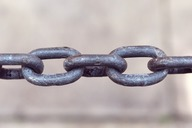
\includegraphics{img/chains.jpg}
\caption[Chains]{Picture from Katrin Baustmann}
\end{figure}
\end{frame}

% picture from
% https://pixabay.com/en/chain-chain-link-border-demarcation-722278/
% Creative Commons CC0

\begin{frame}[fragile]{Chaining / Nesting}
Shallow nesting (chaining)
\begin{lstlisting}
    $rs->search({ name => { '!=', 'blah' }})
        ->search({ name => { '!=', undef }})

    ... WHERE name != 'blah' AND name IS NOT null
Subquery nesting
    $rs->search({}, { distinct => 1 })
        ->as_subselect_rs
         ->search({}, { rows => 1 })

    ... SELECT FROM (SELECT * FROM artist GROUP_BY * ) LIMIT 1
\end{lstlisting}
\end{frame}

\subsection{Correlated Subqueries}
\begin{frame}{Correlated Subqueries}
\end{frame}

\section{Using relationships}
\begin{frame}{Using relationships}
\end{frame}

\section{Extending Schema}
\begin{frame}{Extending Schema}
\end{frame}

\subsection{Using Result Class Components}

In a single result class:

\begin{frame}[fragile]{Using Components}
\begin{lstlisting}
package TravelDance::Schema::Result::User;

use TravelDance::Schema::Candy -components => [qw(
    InflateColumn::DateTime 
    PassphraseColumn
    TimeStamp
)];

\end{lstlisting}
\end{frame}

To add a result class component to all result classes add to list 
in \verb|TravelDance::Schema::Candy|'s \verb|parse_arguments|.

\subsection{Helpers}
\subsubsection{ResultSet Helpers}
\begin{description}
\item[Me] 
simple exact way to set table aliases correctly in queries
\item[Random] small random subset
great for related product searches where you want a small 
random subset of the results
\item[CorrelateRelationship] 
makes correlated subqueries really simple
\end{description}

\begin{frame}{ResultSet Helpers}
\begin{description}
\item[Me] correct table aliases
\item[Random] small random subset
\item[CorrelateRelationship]  
\end{description}
\end{frame}

Problem: we want a count of rows in a related table

Obvious approach:

\begin{lstlisting}
    my $rs = $schema->resultset('Author')->search(
        undef,
        {
            join       => 'books',
            '+columns' => {
                book_count => {
                    count => 'books.id'
                }
            },
            distinct   => 1,    # let DBIC work out group_by for us
        }
    );
\end{lstlisting}

This causes a number of problems:

\begin{itemize}
\item Depending on engine, COUNT’s that aren’t COUNT(*) tend to be slow as
they do table scans.
\item This is hard to chain since we've introduced JOIN and GROUP BY and
collapsed COUNTs might produced unexpected results.
\end{itemize}

\begin{lstlisting}
Much nicer to do:

    package MyApp::Schema::ResultSet::Author;

    use parent 'DBIx::Class::ResultSet';

   
__PACKAGE__->load_components(qw(Helper::ResultSet::CorrelateRelationship));

    sub with_book_count {
        my $self = shift;

        $self->search(
            undef,
            {
                '+columns' => {
                    book_count =>
$self->correlate('books')->count_rs->as_query
                }
            }
        );
    }
\end{lstlisting}

Then elsewhere:

\begin{lstlisting}
my $rs = $schema->resultset('Author')->with_book_count;

The SQL query will look something like this:

  SELECT me.id, me.name, me.foo, ..., (
    SELECT COUNT( * )
      FROM books books_alias
     WHERE books_alias.id = authors.id
   )
  FROM authors me

This is *much* faster and *always* chainable since no JOIN, GROUP BY, or
other junk added to query.
\end{lstlisting}

Cool example from Interchange6::Schema::ResultSet::Product :

\begin{lstlisting}
    sub with_average_rating {
        my $self = shift;

        return $self->search(
            undef,
            {
                '+select' => [
                    {
                        coalesce => [

                            $self->correlate('canonical')
                              ->related_resultset('_product_reviews')
                              ->search_related(
                                'message',
                                { 'message.approved' => 1,
'message.public' => 1 }
                             
)->get_column('rating')->func_rs('avg')->as_query,

                            $self->correlate('_product_reviews')
                              ->search_related(
                                'message',
                                { 'message.approved' => 1,
'message.public' => 1 }
                             
)->get_column('rating')->func_rs('avg')->as_query,

                          ],
                        -as => 'average_rating'
                    }
                ],
                '+as' => ['average_rating'],
            }
        );
    }
\end{lstlisting}

\subsubsection{Shortcuts}
\begin{description}
\item[AddColumns] 
\item[Columns]
\item[Distinct]
\item[GroupBy] 
\item[HRI]
uses this all the time
\item[HasRows] much faster than count for very large resultsets
\item[Limit]
\item[OrderBy]
\item[Page]
\item[Prefetch]
\item[Rows]
\item[Search::{Not}Like]
\item[Search::{Not}Null] 
\end{description}

Using the HashRefInflator makes sense when you need to quickly retrieve
data from a massive resultset or you need a list of hash references anyway,
e.g. for input to a template in a web application.

\begin{frame}[fragile]{HashRefInflator}
\begin{lstlisting}
my $rs = $schema->resultset('Country')->search({}, {
   result_class => 'DBIx::Class::ResultClass::HashRefInflator',
 });
\end{lstlisting}
\end{frame}

\begin{frame}[fragile]{HashRefInflator with HRI helper}
\begin{lstlisting}
my $rs = $schema->resultset('Country')->search({})->hri;
\end{lstlisting}
\end{frame}

\subsubsection{Schema}
\begin{description}
\item[DateTime]
much simpler query construction for DateTime inflated fields
\item[QuoteNames] 
forces quote\_names even if someone misses it in their 
config yml - everyone should use this
\end{description}

\begin{frame}{Schema Helpers}
\begin{description}
\item[DateTime] DateTime inflated fields
\item[QuoteNames] forces quote\_names
\end{description}
\end{frame}

\section{Writing Tests}
\begin{frame}{Writing Tests}
\end{frame}

\section{Deployment Handler}

\begin{frame}{Deployment Handler}
\begin{itemize}
\item DBIx::Class::DeploymentHandler
\item Deploy databases
\item Upgrade databases
\item Downgrade databases
\end{itemize}
\end{frame}

\begin{frame}{Principles}
\begin{itemize}
\item Create backup
\item Change schema
\item Add custom scripts
\item Bump version number
\item Prepare upgrade
\item Deploy upgrade
\end{itemize}
\end{frame}

Note: create backup can be done by DeploymentHandler itself.

\begin{frame}{Change Schema}
\begin{itemize}
\item Add table
\item Add column
\item Alter column
\end{itemize}
\end{frame}

\subsection{Prepare upgrade}
\begin{lstlisting}
my $dh     = DBIx::Class::DeploymentHandler->new(
    {
        schema              => $schema,
        databases           => 'MySQL',
        sql_translator_args => { add_drop_table => 0 }
    }
);
$dh->prepare_deploy;
$dh->prepare_upgrade(
    {
        from_version => $dh->database_version,
        to_version => $dh->schema_version
    }
);
\end{lstlisting}

\subsection{Add custom scripts}

\begin{frame}{Add custom scripts}
\begin{itemize}
\item Add initial values for new tables
\begin{itemize}
\item hardcoded in script
\item from file
\end{itemize}
\end{itemize}
\end{frame}

\subsection{Internals}

\begin{frame}{Directories and files}
\end{frame}

\end{document}

%%% Local Variables: 
%%% mode: latex
%%% TeX-master: t
%%% End: 
